\documentclass[a4j]{ujarticle}
\usepackage[dvipdfmx]{graphicx}
\usepackage{url}
\usepackage{bbding}
\usepackage{lscape}
\usepackage[subrefformat=parens]{subcaption}


\title{進捗報告資料}
\author{安達智哉\\to-adachi@ist.osaka-u.ac.jp}
\date{平成31年1月4日}

\begin{document}
\maketitle

\section{CPUとメモリ間で負荷をオフロードするモデル}

\subsection{概要}
\label{sec:abs}
MMEおよびSGW、PGWなどのEPCノードは、主なリソースとしてCPUとメモリを持っている。CPUは、アタッチやデタッチなどのシグナリング処理を実行するために必要とされるリソースである。一方メモリは、ベアラなどのセッション情報を保持するために必要とされるリソースである。これらのリソースは、モバイルネットワークにおける通信を可能にするために必須であるため、ネットワーク事業者は、どちらのリソースも枯渇することがないように、CPUとメモリをバランスよく割り当てる必要がある。

その一方で、近年はM2M/IoT端末の急激な増加が注目されている。M2M/IoT端末は通信特性において従来の端末(携帯電話やスマートフォン)とは大きく異なり、データの送信に周期性や間欠性を持つという特徴がある。また、M2M/IoT端末は消費電力を抑えることを目的に、データの送信ごとにデタッチ処理を実行し、セッションを解放する特徴がある。この点においても、ネットワークから切り離されるまで、セッションを維持し続ける従来の端末とは異なる。

上述のM2M/IoT端末の特性は、CPUとメモリのバランスの良い割り当てを難しくすると考えられる。なぜなら、M2M/IoT端末はその通信特性から、多くのアタッチ処理およびデタッチ処理を引き起こし、CPU負荷のみを増加させるため、従来の端末と比較すると、CPUとメモリに与える負荷の割合が異なるからである。また、IoT端末の接続台数の予測が難しいこともリソースの割り当てを難しく一因である。IoT端末は、スマートフォンのような従来の端末とは異なり、家電や自動車、電気メーター、センサーなど様々な場所、様々な用途で使用される可能性があり、端末の台数およびその分布を予測することは困難であると考えられる。このように、通信特性が異なり、接続台数の予測が難しいIoT端末の普及により、今後のネットワーク事業者は、CPUとメモリのバランスの良い割り当てがより難しいくなると予想される。

上述のようなネットワーク(CPUとメモリのリソース消費の予測が難しく、変動が激しいネットワーク)において、収容可能な端末の増加を目的とした既存研究には、スケールアウトの考え方を用いたものが多い。これらの研究では主に稼働するサーバやインスタンスの数をリソースの需要に応じて変動させることにより、ネットワークの変動に対応している。しかし、この方法では、本来必要とされているリソース量(需用量)よりも多くのリソースが供給される、リソースの過剰分配が発生する問題がある。なぜなら、これらの研究では、サーバやインスタンス一台あたりのリソース量は一定であることが前提の研究が多く、細かい粒度でリソースを制御できないためである。また、必要とされるCPUとメモリのリソース比はあらかじめ分かっている前提の研究が多く、必要とされるリソース比が未知の場合はリソースの効率的な利用ができないからである。例えば、CPUのリソース不足を解消するためにケールアウトを行った場合、CPUリソースと同時にメモリリソースも増加する。しかし、メモリは元々ボトルネックにはなっていないため、新たに追加されたメモリは過剰分配されたことになる。


このような背景から、CPUとメモリのリソース消費の予測が難しような状況や変動が大きいような状況においても、どちらかがボトルネックにならずに、効率的にリソースを活用するアーキテクチャを考えることは重要である。実際、CPUとメモリのリソースを効率よく活用する研究は、データセンターなどの分野では行われている。しかし、モバイルネットワークに特化した研究は行われていない。そこで、私はモバイルネットワークに特化した、CPUとメモリのリソースのオフロードを可能にする仕組みを考えた。この方法により、CPUが過負荷である場合は、メモリの負荷を増加させる代わりにCPUの負荷を削減することが可能である。またその逆に、メモリが過負荷である場合は、CPUの負荷を増加させることによりメモリの負荷を削減できる。この仕組みにより、CPUとメモリのリソース消費の予測が難しい場合や、変動が激しいネットワークであっても、CPUおよびメモリ双方のリソース利用率の向上が期待でき、収容可能な端末の増加が期待できる。

% 私の案は、本来ならデタッチ処理が行われるタイミングであってもあえてデタッチ処理を行わないようにすることである。つまり、M2M/IoT端末がデータの送信を終え、電源をOFFにした後も、一部のセッションはそのまま維持しつつける。そして、M2M/IoT端末が再びONになりデータを送信する際には、以前と同じベアラを用いてデータを送信する。この方法によって、最初に一度アタッチ処理を行えば、その後のデータ送信においては、アタッチ処理は発生しないで済むため、アタッチおよびデタッチ処理を行うために必要なCPU負荷を削減しすることが可能である。
% 一方、本来は解放されるはずのセッション情報を維持し続けるため、その分メモリへの負荷が大きくなる。メモリのリソースが不足し、CPUリソースに余裕がある場合は、デタッチ処理が発生するまでの時間を短くすることにより、ベアラを維持するために必要なメモリリソースを積極的に解放してメモリ負荷を削減する。一方、その分デタッチ、アタッチ処理が頻繁に発生するため、CPUへの負荷は大きくなる。

\subsection{負荷について}
\subsubsection{CPU負荷}
CPU負荷は、主にアタッチやデタッチなどのシグナリング処理を各ノードで実行する際に発生する。時間当たりのシグナリング処理の実行回数の増加に伴い、負荷が増加する。CPU負荷の増加は、各ノードにおける処理時間の増大を引き起こす。また、CPUが過負荷状態になると、それ以上のシグナリング処理の実行が困難になる。
\subsubsection{メモリ負荷}
メモリ負荷は、主にベアラなどのセッションを維持するために必要な情報(ベアラ識別子、UE情報、ステート情報など)を保持する際に発生する。維持するベアラの増加に伴い、負荷が増加する。メモリが過負荷状態になると、新しくベアラを確立するために、古いベアラを解放する必要がある。
\subsubsection{負荷のオフロードについて}
負荷のオフロードに関するイメージ図を図\ref{cpu}および図\ref{memory}に示す。各図は端末台数とCPUおよびメモリリソースの使用率の関係をそれぞれ赤および青の線で示している。端末台数とは、システムが収容しているUEの数である。リソースの使用率とは、システムが利用できるリソースの最大値(物理的な性能の限界値や、事前にオペレータが設定した閾値などが想定される)に対して、UEを収容するために割り当てる必要のあるリソース量の割合である。一台あたりのUEを収容するために必要なリソース量の平均値はグラフの傾きに表れており、この値はUEの通信特性に応じて変化する。

図\ref{cpu}は、メモリリソースと比較してCPUリソースを大きく消費するような通信特性を持つUEを収容した場合のグラフである。図\ref{cpu}(a)を見ると、端末台数が$a$台の時点でCPU使用率が100\%に達していることがわかる。そのため、収容可能なUEの台数は$a$台である。一方、図\ref{cpu}(b)では、第\ref{sec:des}節で述べる方法により、一台あたりのUEを収容するために必要なリソース量を変化させた場合のモデルである。この図の例では、ボトルネックであったCPUの負荷をメモリにオフロードすることにより、収容可能な端末台数が$a$台から$a'$台に増加している。このように、CPUリソースが不足し、メモリリソースが余っているような場合においては、CPUの負荷をメモリにオフロードすることにより収容可能なUEの台数が増加する可能性がある。

同様にCPUリソースが余っている状態で、メモリが枯渇した場合においては、メモリからCPUへ負荷をオフロードすることにより、収容可能なUEの台数が増加する(図\ref{memory})。





\begin{figure}[p]
	\centering
		\begin{subfigure}{1.0\textwidth}
			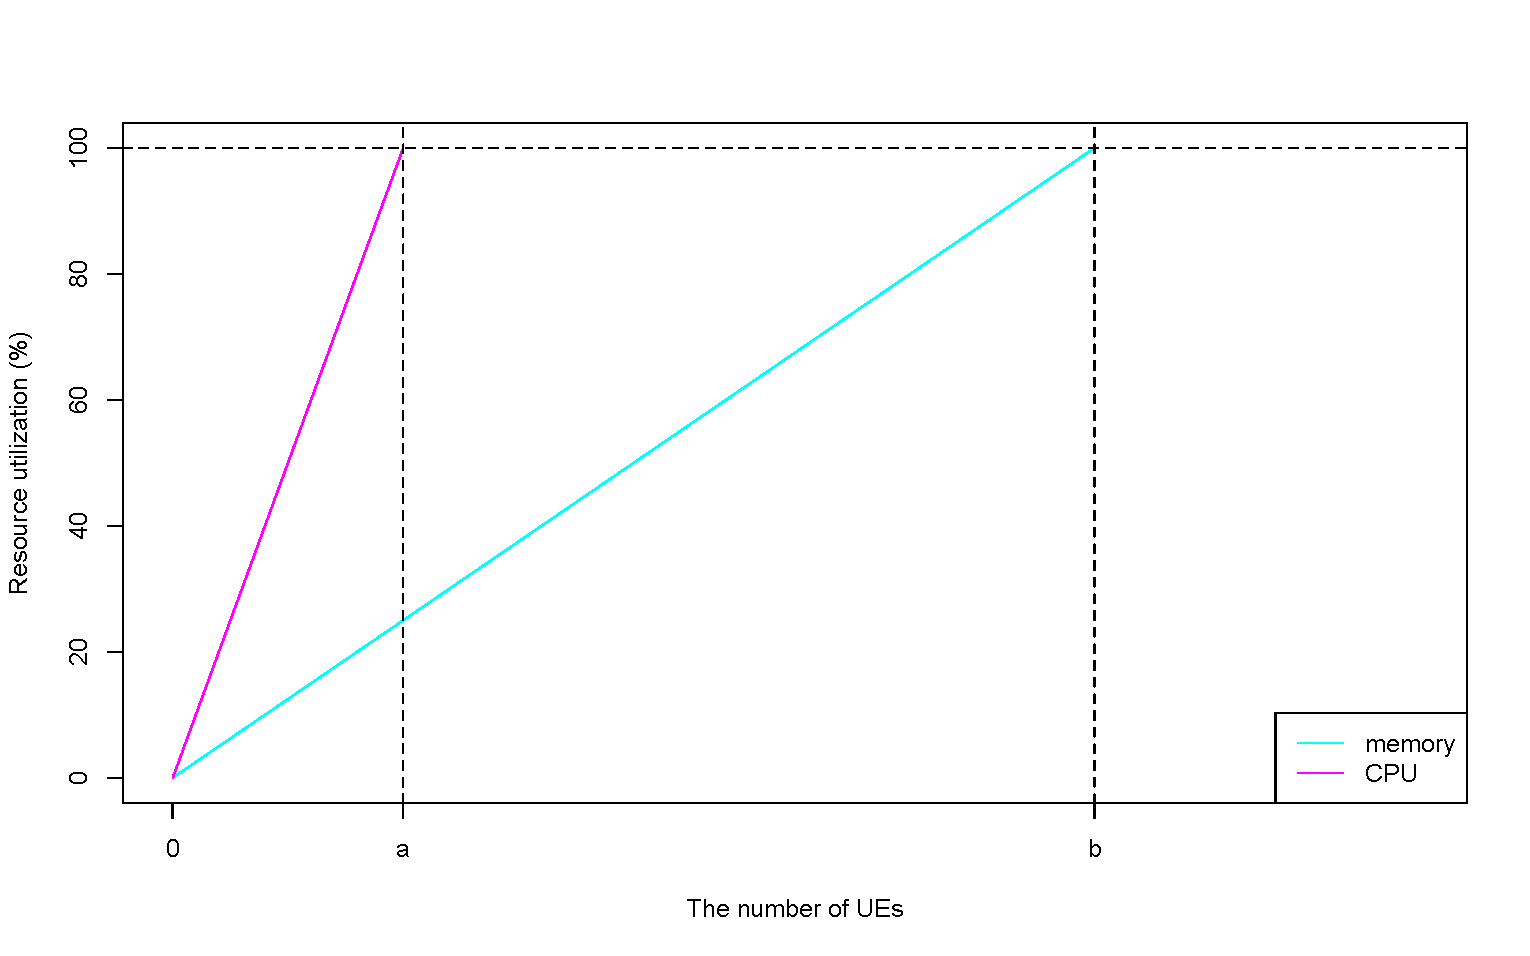
\includegraphics[width=1.0\hsize]{plot1.pdf}
			\caption{オフロードを行わない場合}
			\label{overcpu}
		\end{subfigure}
		\begin{subfigure}{1.0\textwidth}
			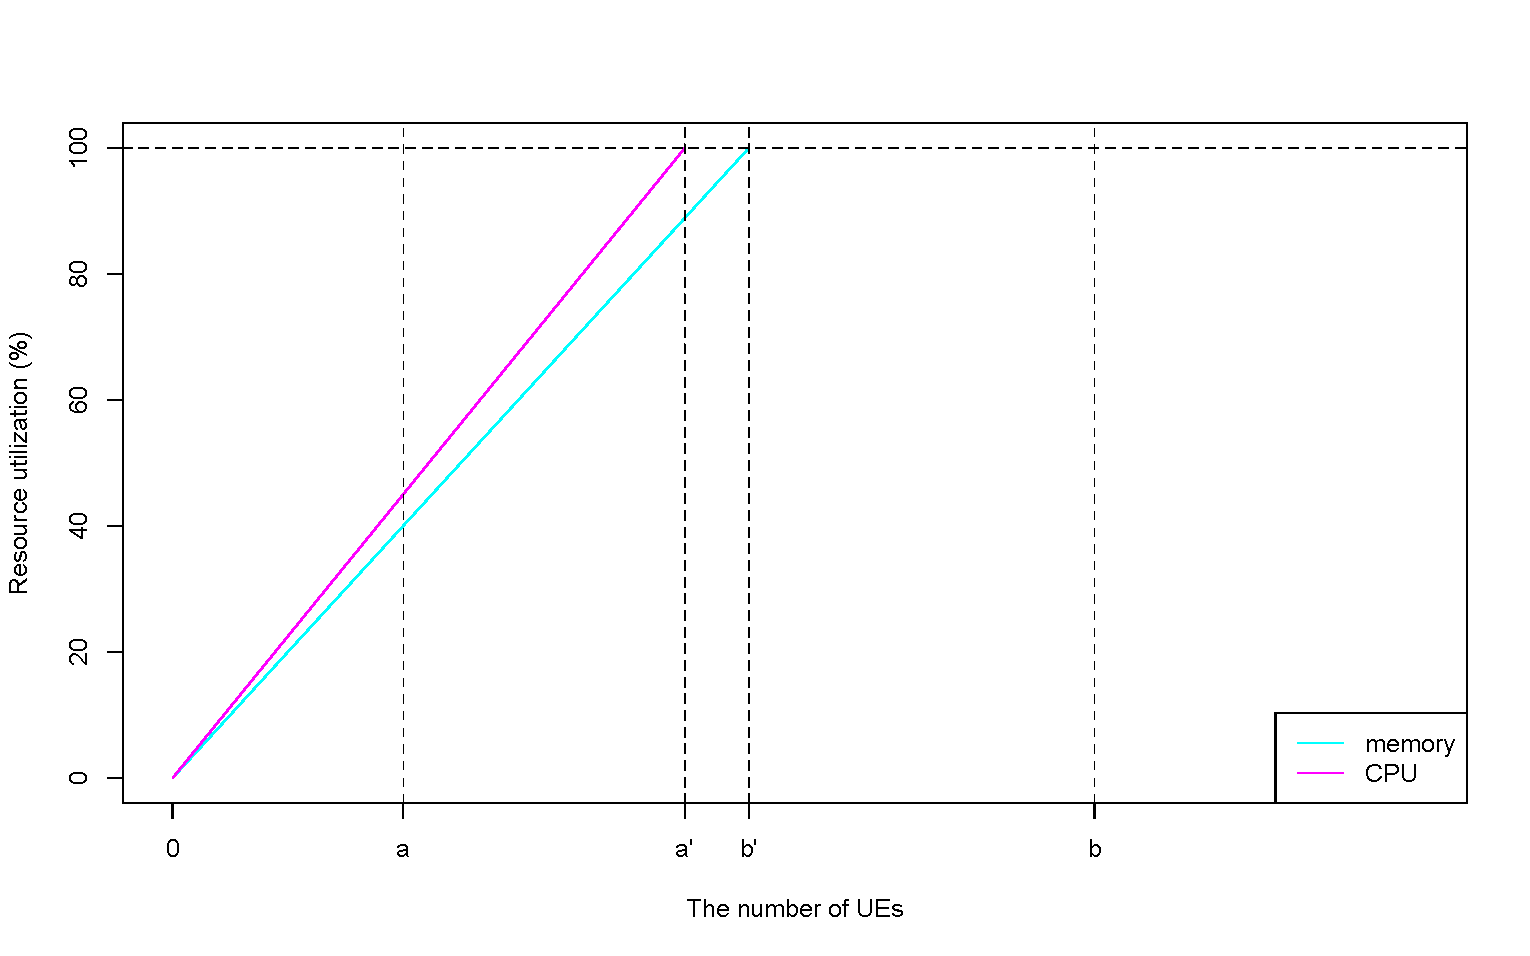
\includegraphics[width=1.0\hsize]{plot2.pdf}
		  \caption{オフロードを行った場合}
			\label{okcpu}
		\end{subfigure}
		\caption{CPU負荷をメモリへオフロード}
		\label{cpu}
\end{figure}


\begin{figure}[p]
	\centering
		\begin{subfigure}{1.0\textwidth}
			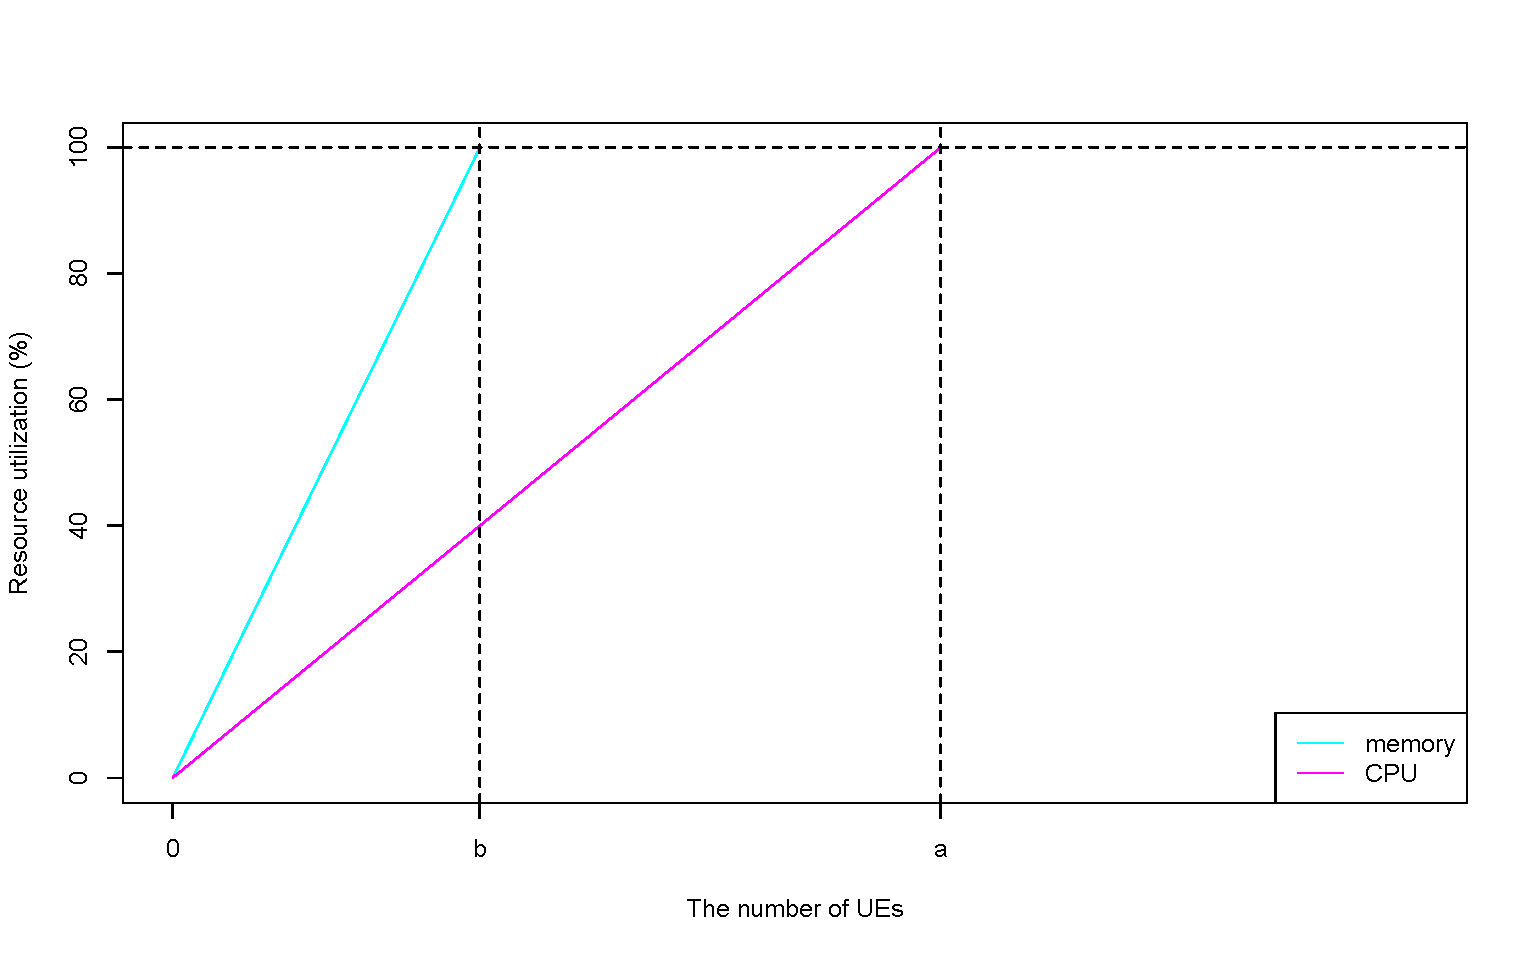
\includegraphics[width=1.0\hsize]{plot3.pdf}
			\caption{オフロードを行わない場合}
			\label{overmemory}
		\end{subfigure}
		\begin{subfigure}{1.0\textwidth}
			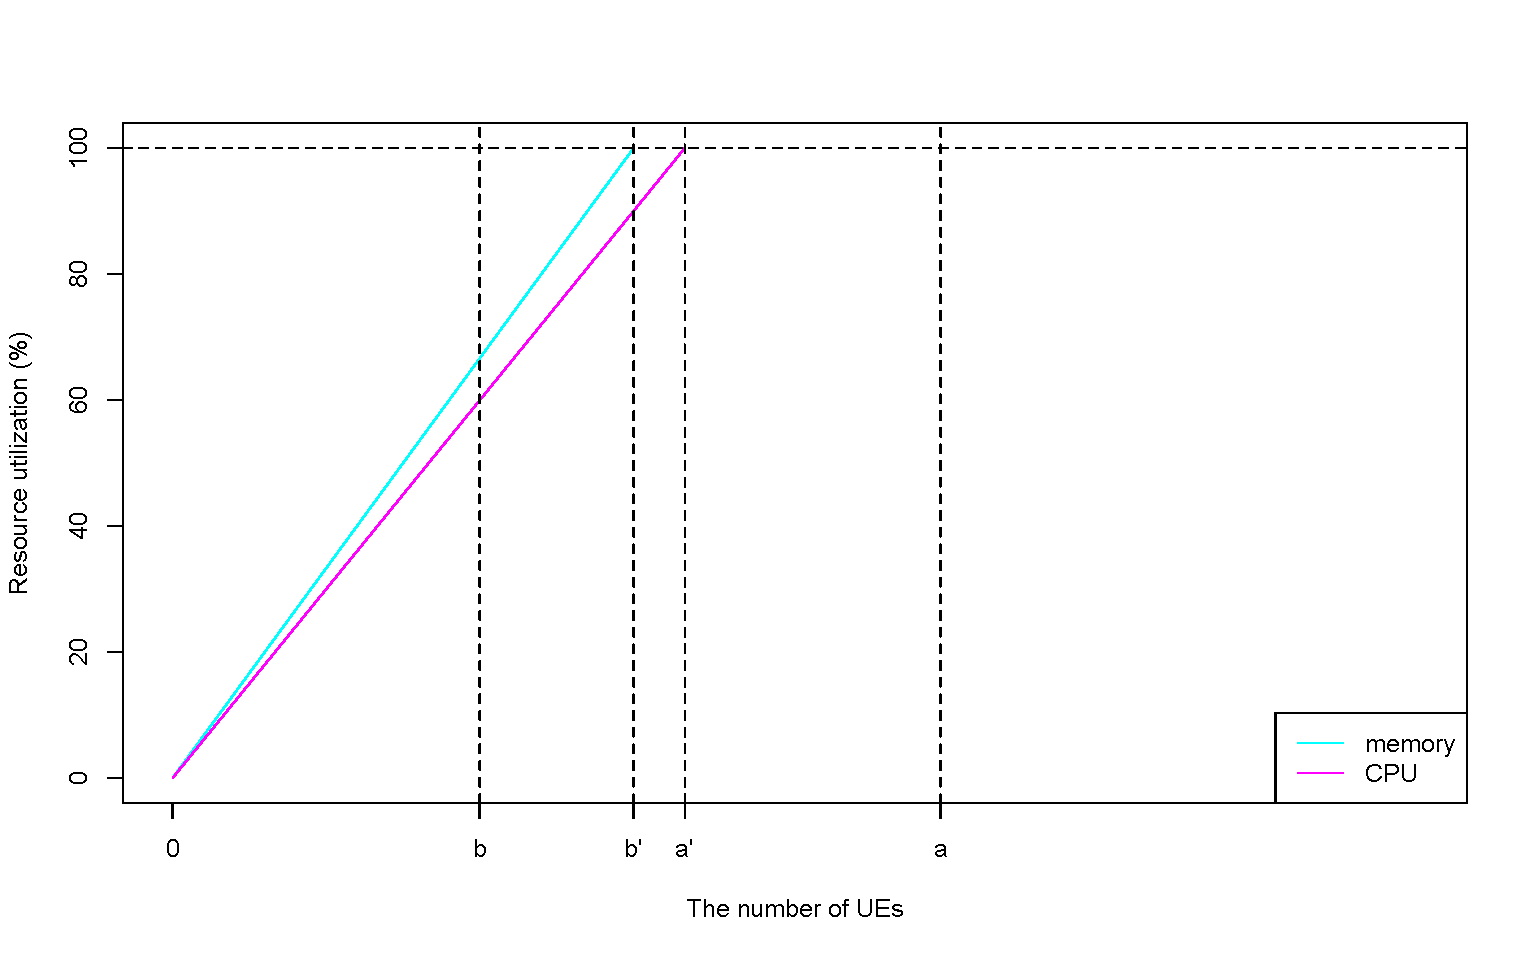
\includegraphics[width=1.0\hsize]{plot4.pdf}
		  \caption{オフロードを行った場合}
			\label{okmemory}
		\end{subfigure}
		\caption{メモリ負荷をCPUへオフロード}
		\label{memory}
\end{figure}
%
%
% \begin{figure}[htbp]
% 	\centering
% 	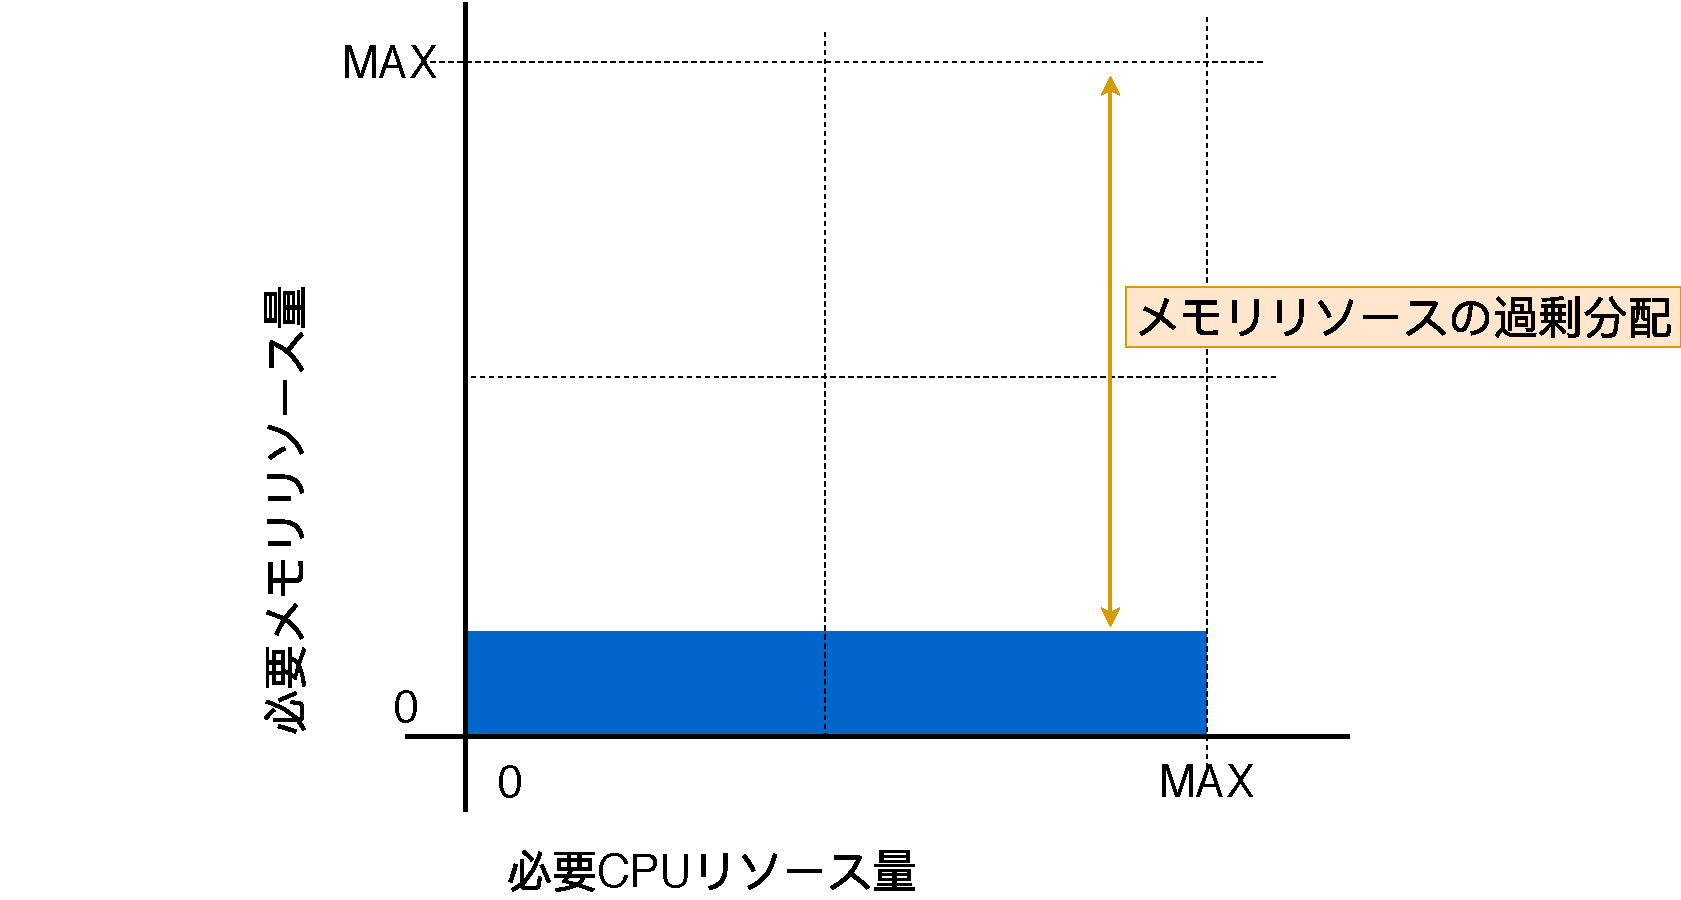
\includegraphics[width=0.8\hsize]{scaleout.pdf}
%   \caption{スケールアウトによるリソース増強}
% 	\label{scaleout}
% \end{figure}

\clearpage
\subsection{負荷のオフロード方法}
\label{sec:des}
通常、UEがネットワークから切り離されたあと、デタッチ処理が行われるまでの時間($t$)は一定である。私は、この$t$を変化させることによって、CPUとメモリの間で負荷をオフロードできるのではないかと考えた。
図\ref{detach-ON}は、M2M/IoT端末が最初にネットワークに接続した際の様子を示したものである。通常通り、アタッチの処理を行い、ベアラを確立する。図\ref{detach-OFF}は、M2M/IoT端末がネットワークから切断された際の様子である。通常は、数秒後にデタッチ処理が行われ、ベアラは全て解放されるが、このモデルでは、$t$を非常に長く設定している。そのため、デタッチ処理が行われないため、ベアラはそのまま維持される(UE-eNodeB間の無線帯域は解放する)。図\ref{detach-reON}はM2M/IoT端末が再びネットワークに接続した時の様子を示す。この場合、以前使用したベアラが残っているため、M2M/IoT端末は無線部分以外のアタッチ処理をスキップしてデータの送受信を開始できる。結果的に、EPCノードで行うアタッチ処理およびデタッチ処理の回数が削減されるため、CPUに与える負荷が削減される。一方、ネットワークに接続されていないM2M/IoT端末のセッション情報を保持する必要があるため、メモリが圧迫されることが予想される。

逆もまた同様であり、メモリリソースが不足した場合は、$t$を短く設定することにより、セッション情報を保持する時間を短くすることができ、メモリの負荷を削減できる。一方、アタッチおよびデタッチ処理が頻発するため、CPU負荷が増加することが予想される。


\begin{figure}[htbp]
	\centering
	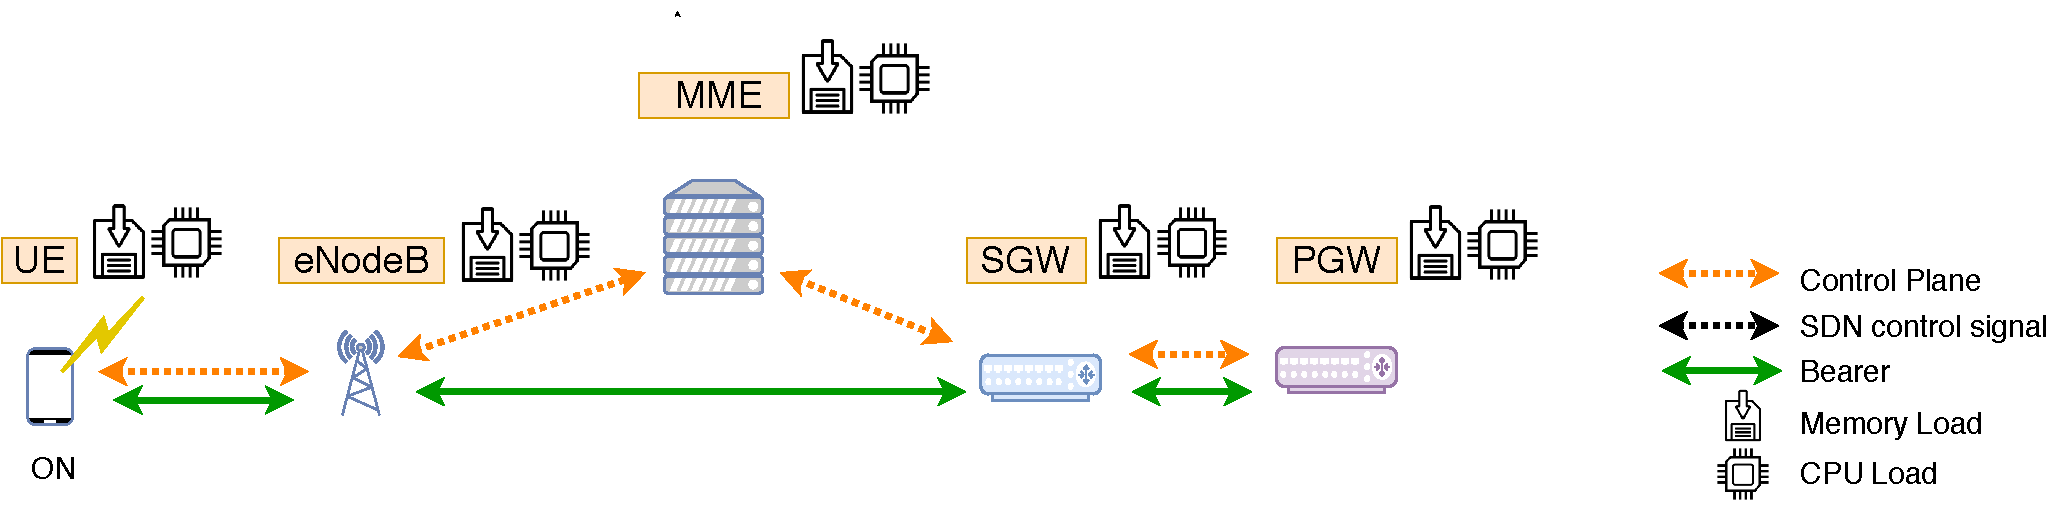
\includegraphics[width=0.7\hsize]{detach-ON.pdf}
  \caption{端末が最初にネットワークに接続した時と処理}
	\label{detach-ON}
\end{figure}

\begin{figure}[htbp]
	\centering
	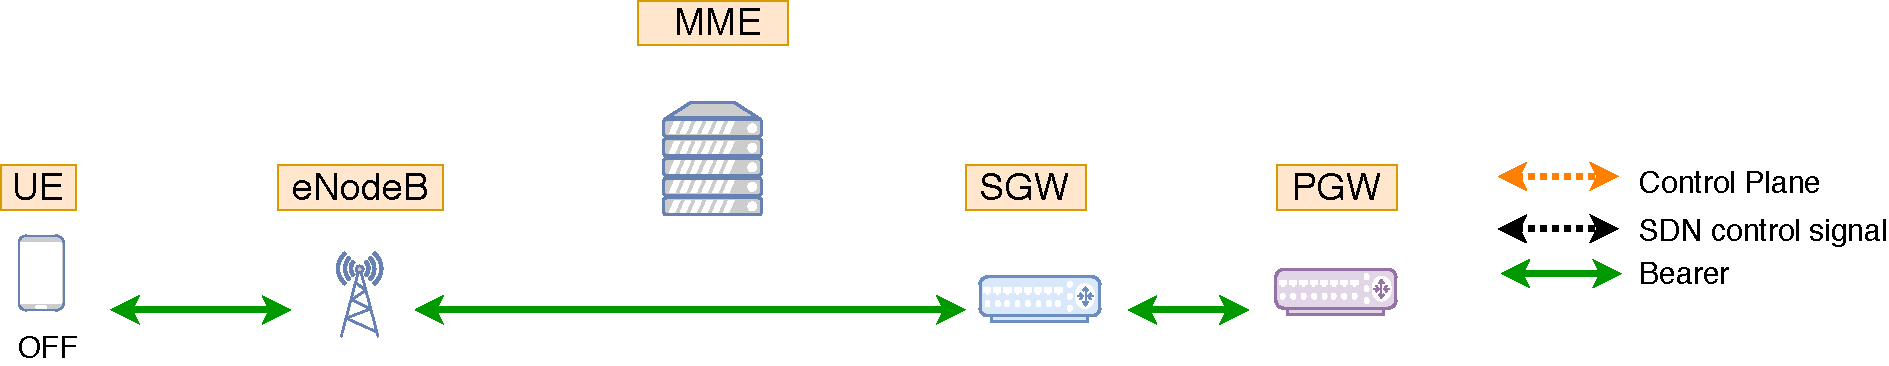
\includegraphics[width=0.7\hsize]{detach-OFF.pdf}
  \caption{端末がネットワークから切り離された時の処理}
	\label{detach-OFF}
\end{figure}

\begin{figure}[htbp]
	\centering
	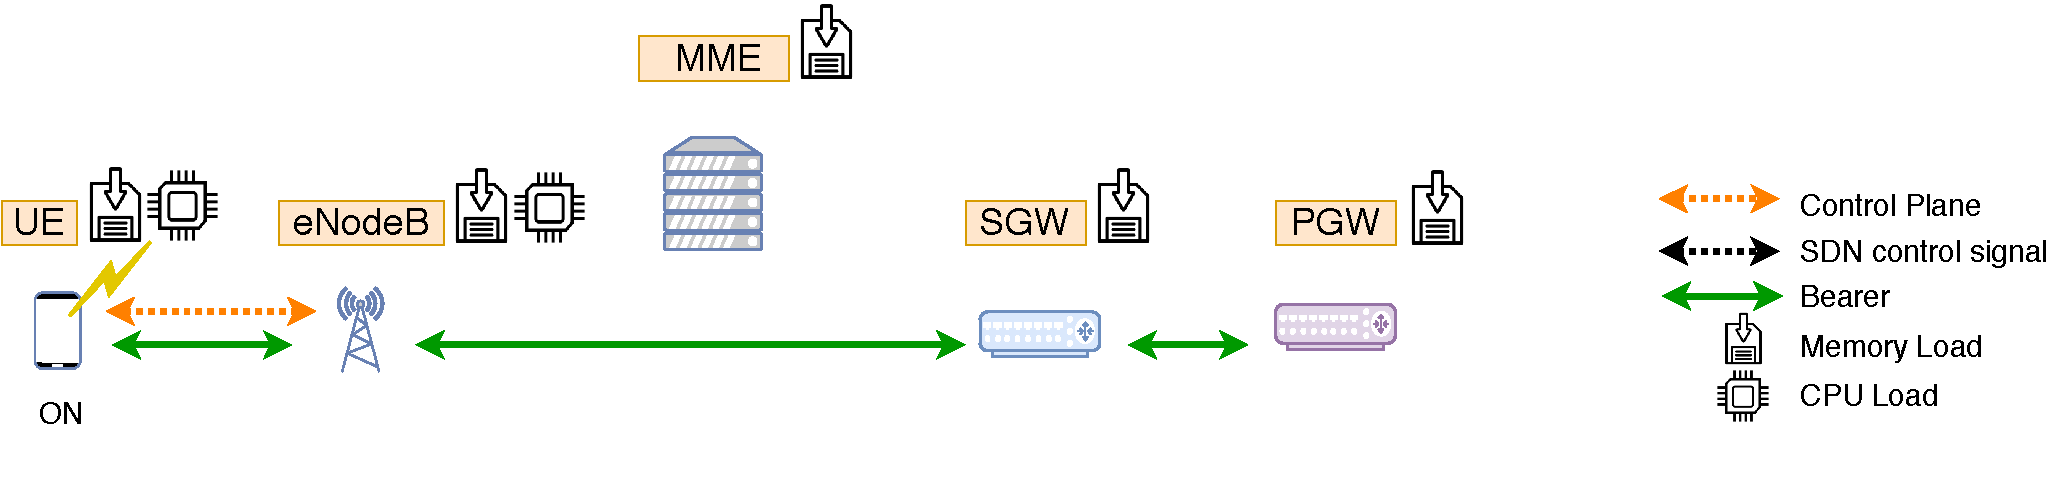
\includegraphics[width=0.7\hsize]{detach-reON.pdf}
  \caption{端末が2回目以降にネットワークに接続した時の処理}
	\label{detach-reON}
\end{figure}

\section{今後の研究について}
\subsection{ネットワークモデル}
これまでは、広域モバイルネットワークを対象とした評価を行ってきたが、今回は(まずは)単一のEPCで構成されるモバイルネットワークを対象とした評価を行うことを考えている。
\subsection{CPU負荷について}
CPUにかかる負荷はこれまで行ってきた研究と同様に、アタッチ処理のプログラム行数に基づく待ち行列理論で求めようと考えている。待ち行列理論によって導出される処理遅延時間が一定の閾値を超えた場合に、CPUリソースが不足したとみなす。
\subsection{メモリ負荷について}
メモリの負荷に関しては、確立しているベアラの数に比例した負荷がかかると仮定する。ベアラの数が閾値を超えた場合に、メモリリソースの不足が発生するものとする。
\section{今後の課題}
第\ref{sec:abs}節で述べた内容の根拠を示す参考文献を探す。
% \section*{\addcontentsline{toc}{section}{参考文献}}
% {\scriptsize
% \bibliographystyle{IEEEtran}
% \bibliography{/Users/t-adachi/Documents/study/Bibliography/bib/hpt_core_network/myBib/LABbiblio,/Users/t-adachi/Documents/study/Bibliography/bib/hpt_core_network/Study_Group_Bibtex/bib/hptCoreNetwork_Study}
% }
\end{document}

%
% \begin{figure}[p]
% 	\centering
% 		\begin{subfigure}{1.0\textwidth}
% 			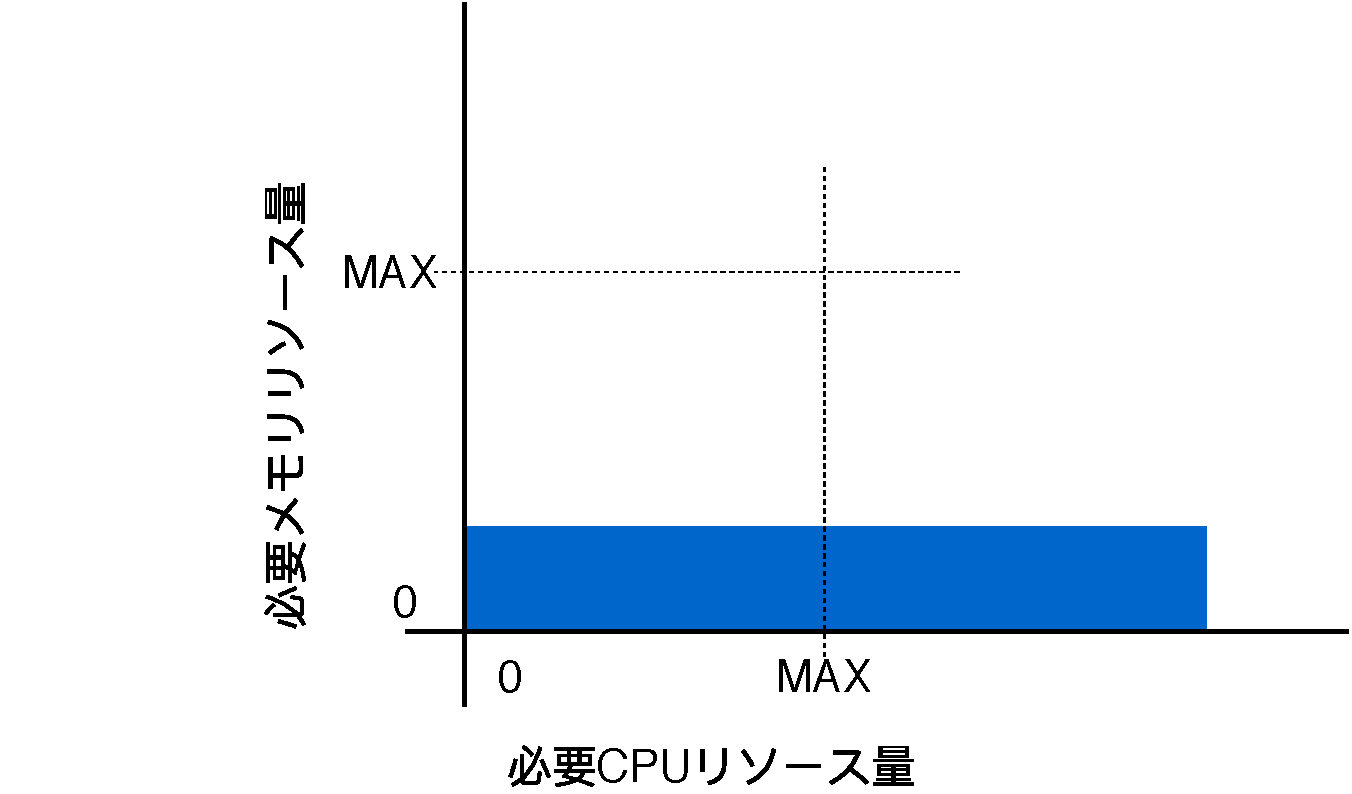
\includegraphics[width=0.8\hsize]{overcpu.pdf}
% 			\caption{オフロードを行わない}
% 			\label{overcpu}
% 		\end{subfigure}
% 		\begin{subfigure}{1.0\textwidth}
% 			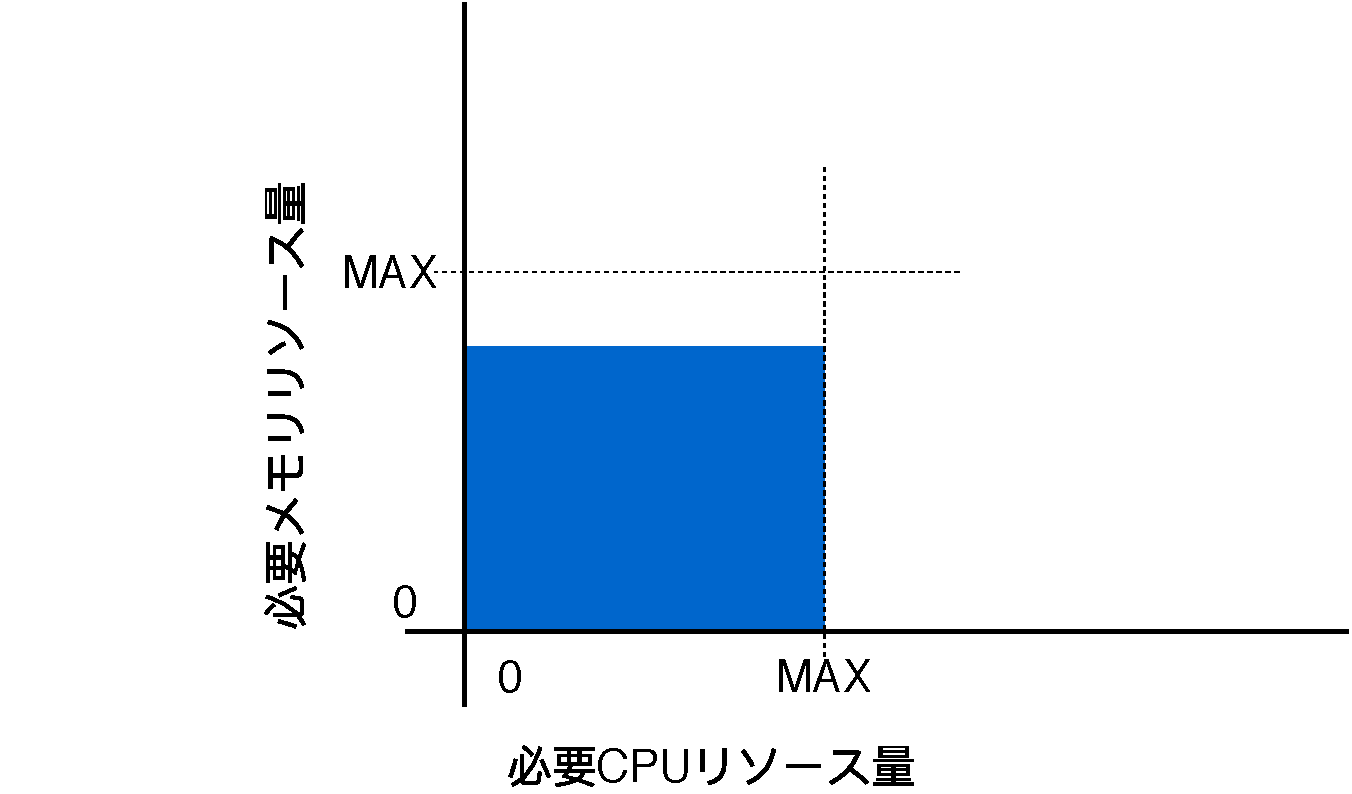
\includegraphics[width=0.8\hsize]{okcpu.pdf}
% 		  \caption{オフロードを行った場合}
% 			\label{okcpu}
% 		\end{subfigure}
% 		\caption{CPU負荷をメモリへオフロード}
% 		\label{cpu}
% \end{figure}
%
%
% \begin{figure}[p]
% 	\centering
% 		\begin{subfigure}{1.0\textwidth}
% 			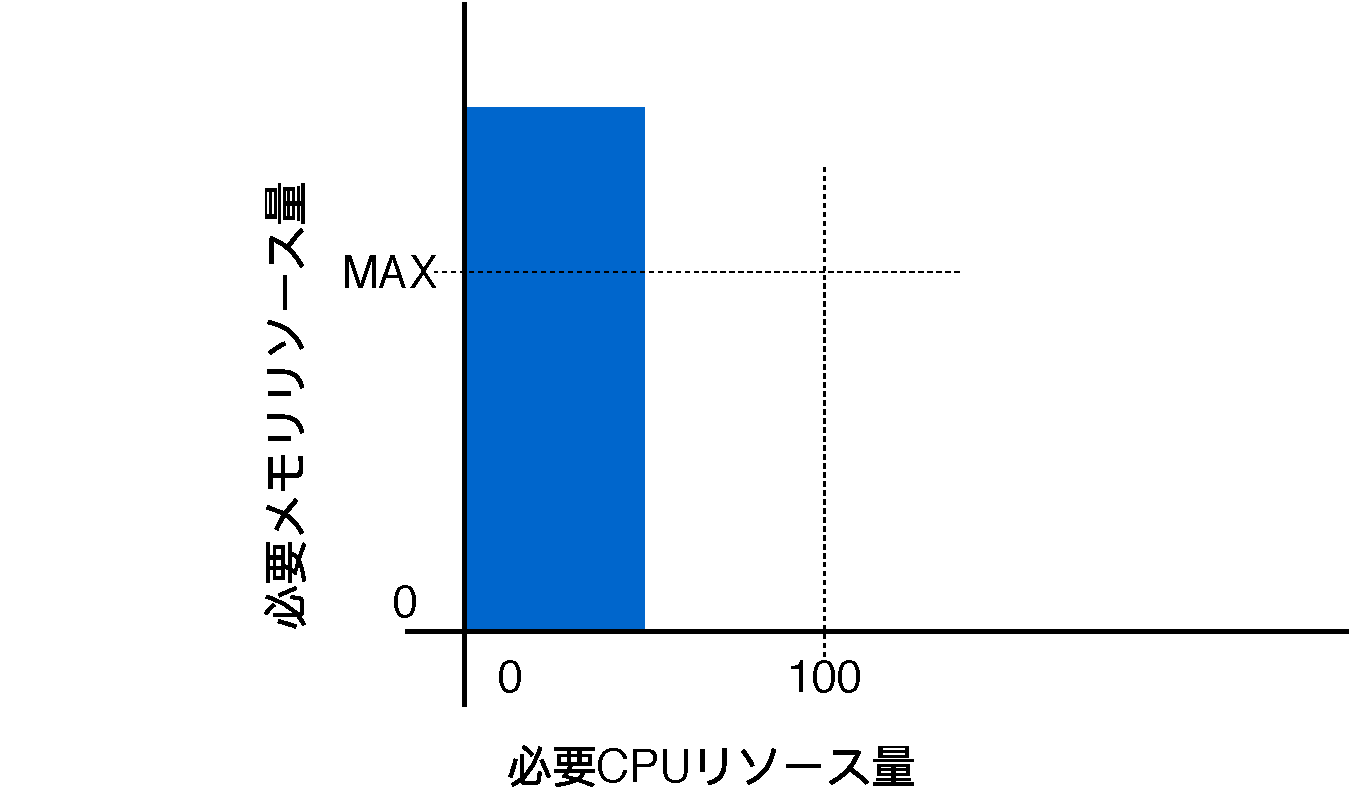
\includegraphics[width=0.8\hsize]{overmemory.pdf}
% 			\caption{オフロードを行わない場合}
% 			\label{overmemory}
% 		\end{subfigure}
% 		\begin{subfigure}{1.0\textwidth}
% 			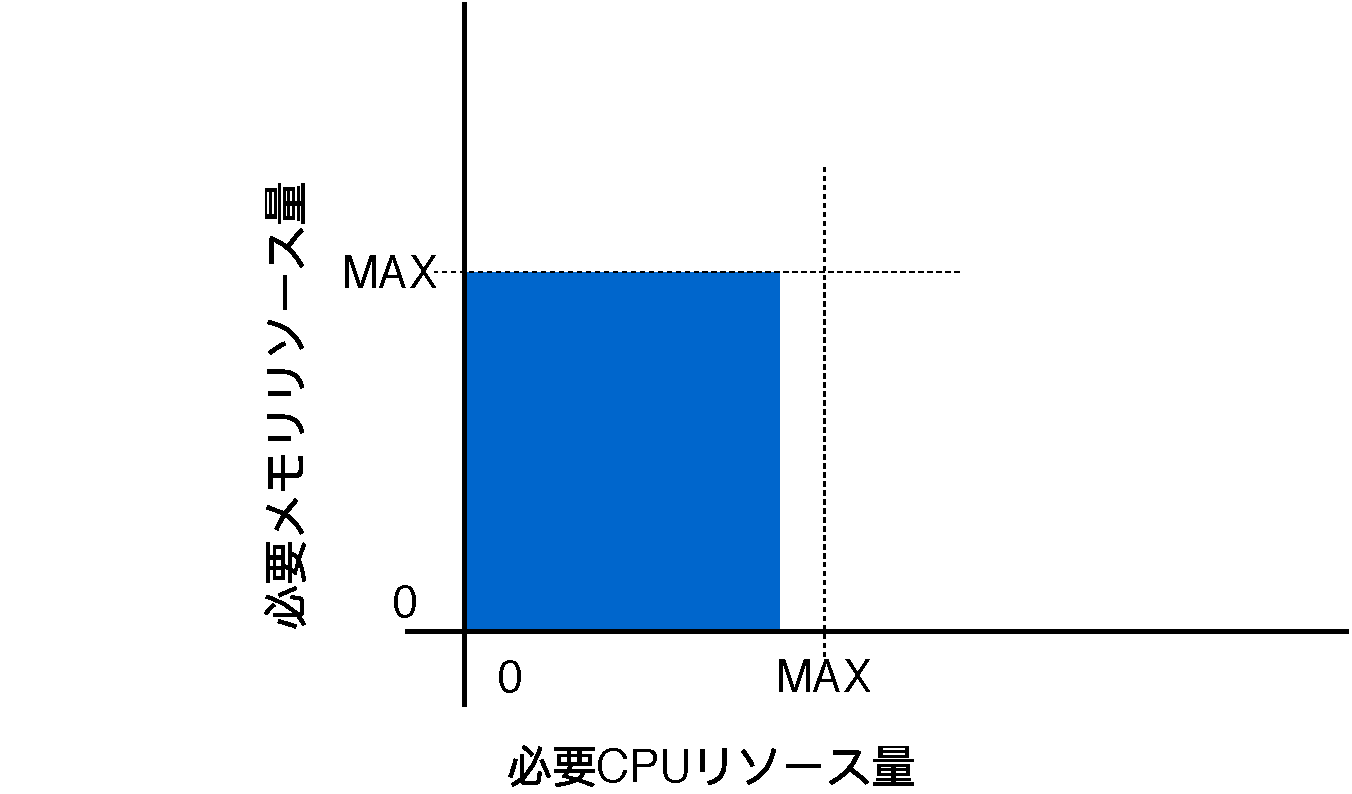
\includegraphics[width=0.8\hsize]{okmemory.pdf}
% 		  \caption{オフロードを行った場合}
% 			\label{okmemory}
% 		\end{subfigure}
% 		\caption{メモリ負荷をCPUへオフロード}
% 		\label{memory}
% \end{figure}
